The additional constants $h$ and $T_inf$ must be added to the System class:
\begin{lstlisting}
sys.add_constant('k',2,'A',0.1,'b',5,'q_bar',5,'h',0.1,'T_inf',10); 
\end{lstlisting}

The convective term contributes to both the stiffness matrix and force vector, thus an additional matrix and vector must be added to the System.
\begin{lstlisting}
sys.add_matrix('K_h', 'N''*h*N');
sys.add_vector('f_h', '-T_inf*N''',1);
\end{lstlisting}

These newly created terms must be added to the assembled stiffness matrix and force vector.
\begin{lstlisting}
K = sys.assemble('K') + sys.assemble('K_h');
f = sys.assemble('f_s') + sys.assemble('f_q') + sys.assemble('f_h');
\end{lstlisting}

Since there are no explicitly defined essential boundary conditions, only the mixed convective boundary, the solution for temperatures is done using the complete stiffness matrix and force vector.
\begin{lstlisting}
T = K\f;
\end{lstlisting}

The resulting temperatures are -21.0, 36.9, and 42.3 \C ~for the left, middle, and right of the bar.
\begin{center}
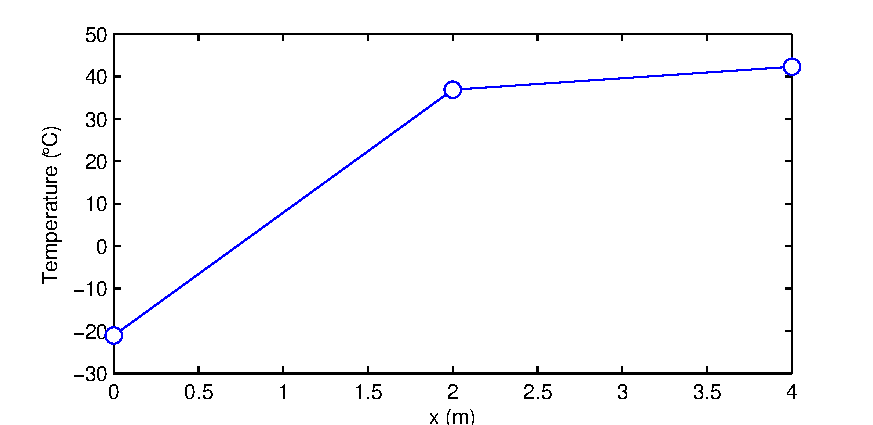
\includegraphics{HW2/HW2-2/soln.pdf}
\end{center}